\documentclass{backend}
\begin{document}

%-------------- Init --------------

\buildmargins       % build page structure
\firstPage          % build cover page
\summary    	    % build summary

%-------------- Body --------------
  

\section{Introduction}

\commentaire{
Dans l'Histoire, la signature est un mécanisme qui remonte au moins à 3100 avant J.C \cite{sumer_sign}. On a pu observer sur des tablettes de gestion de blé, de la cité sumérienne d'Uruk, le nom "Kushim". Cette signature permet d'affirmer une identité à un travail, un auteur à un écrit... En revanche, les historiens considèrent que cette marque n'est pas encore une signature et que c'est plutôt durant l'Antiquité que la signature devient moderne. Elle devient un moyen de distinguer et d'authentifier des documents.\medbreak

Désormais à l'ère informatique, la signature se transpose au numérique. Premièrement

La signature numérique a été décrite par Whitfield Diffie et Martin Hellman en 1976 \cite{1055638} sur l'idée de fonctions à sens unique à trappe, c'est en 1978 dans \citetitle{signRSA} \cite{signRSA} que Ronald Rivest, Adi Shamir et Leonard Adleman ouvrent la voie pour une première implémentation.\medbreak

Pour être utile, une signature numérique doit posséder les propriétés suivantes :
\begin{itemize}
  \item Authentification : l'identité du signataire doit pouvoir être retrouvée de manière certaine
  \item Infalsifiable : une signature ne peut pas être reproduite
  \item Unique : la signature dépend du document signé et ne peut être appliquée sur un autre document
  \item Inaltérable : une fois un document signé, on ne peut plus le modifier
  \item Irrévocable : la personne qui signe ne peut le contester
\end{itemize}\medbreak

Ainsi, lorsque de nouveaux protocoles de signatures numériques sont proposés, il est nécessaire de vérifier la robustesse de ces propriétés. Le NIST (National Institute of Standards and Technology) ou encore les PKCS (Public Key Cryptography Standards) de RSA Security sont considérés comme les organismes de référence pour les standards de protocoles. Une implémentation d'algorithme de signature qui suit leurs standards peut être considérée comme fiable.  La signature DSA (FIPS 186 du NIST) était un de ces standards. Elle fut mise au point en 1991 à partir des cryptosystèmes de Schnorr et ElGamal \cite{dsaFIPS} et utilisée dès 1994. Cependant, elle est considérée comme obsolète depuis 2023. En effet, maintenir un bon niveau de sécurité en l'utilisant aujourd'hui demanderait des entiers d'au moins 3072 bits. Un grand manque d'efficacité et de performance quand on compare avec sa version plus compacte. Cette dernière utilise des groupes de points sur courbe elliptique, ce qui lui donnera son nom, ECDSA \cite{ecdsaFIPS}. Elle est actuellement très largement répandue, dans la librairie OpenSSL ou dans les protocoles Bitcoin par exemple, ce qui rend les études de sécurité plus importantes.\medbreak
\newpage
}



Ce \subject\:  s'est déroulé de janvier à février dans le cadre de notre master 2 à l'Université de Bordeaux. Il est basé sur l'article de Howgrave-Graham et Smart \cite{latAtk}, publié en 1999, repris en 2001 dans l'ouvrage \textit{Designs Codes and Cryptography}. Dans ce but, nous avons conçu des outils informatiques, développés en \textit{SageMath}, qui nous ont permis d'évaluer et tester nos hypothèses.

\begin{enumerate}
\item Un générateur de paramètres DSA
\item Un générateur de signatures et de traces pour tous les protocoles étudiés
\item Les fonctions de l'attaque de notre référence
\item Un programme pour filtrer et agréger les résultats avant de les tracer avec \textit{numpy}, \textit{pandas}, \textit{matplotlib} et \textit{seaborn}

\end{enumerate}


Ces outils ont été conçus pour être les plus modulables possibles afin de couvrir de nombreux paramètres et simuler une grande variété d'attaques par canal auxiliaire. \medbreak

Nous avons ajouté des tests automatiques et des outils de visualisation pour comparer les performances de différents algorithmes et effectuer des statistiques. L'ensemble de la partie programmation de ce projet peut être consulté ici :
\begin{center}
    \url{https://gitlab.emi.u-bordeaux.fr/pachauveau/ecdsa}
\end{center}

L'attaque a été conçue pour la signature standard DSA pourtant nous verrons qu'il est possible de l'appliquer facilement à un autre standard ECDSA, sans remettre en cause les propriétés cryptographiques de celui-ci. En effet, cette attaque requiert de l'information sur les bits des clés éphémères utilisées lors de plusieurs signatures. Elle s'inscrit dans le cadre des attaques par canal auxiliaire.


\section{Préambule} \label{sec:preambule}

Cette attaque emploie les réseaux euclidiens. Nous couvrons ici quelques notions utiles pour la compréhension de ce document et présentons les signatures DSA et ECDSA.

\subsection{Réseau Euclidien}

Rappelons d'abord qu'un réseau $L$ est un sous-groupe discret de $\mathbb{R}^n$. Cette structure peut être décrite par une base $\mathcal{B}$ de $d$ vecteurs indépendants \{$b_1, \dots b_d$\} et n'importe quel point du réseau s'exprime comme combinaison linéaire entière de ces vecteurs. En posant $A$ la matrice dont les lignes sont les $d$ vecteurs de $\mathcal{B}$, on peut écrire que $L = \{\mathbf{x}A : \mathbf{x} \in \mathbb{Z}^n\}$\smallbreak

Le Closest Vector Problem ou CVP consiste, pour un réseau $L$ donné et un certain vecteur $t$ de $\mathbb{R}^n$, à retrouver le vecteur de $L$ le plus proche de $t$. Ce problème est connu pour être NP-difficile ce qui implique que la recherche de la solution n'est a priori pas possible en temps polynomial. Pour fonctionner en un temps raisonnable, il est d'usage de trouver une base de $L$ la plus orthogonale possible avec des vecteurs les plus courts possibles. Une telle base est dite réduite et on peut en obtenir d'assez 'satisfaisantes' en utilisant LLL. L'algorithme de Lenstra–Lenstra–Lovász \cite{lll} se base sur le procédé de Gram-Schmidt pour orthogonaliser les vecteurs de la base.\smallbreak


Plus la base est réduite, plus les algorithmes comme celui de Babai sont efficaces pour trouver un vecteur de $L$ proche de notre vecteur cible $t$. Nous détaillons un peu plus en annexe \ref{annexe:Babai} le fonctionnement de cet algorithme ainsi que ses différentes versions.\smallbreak


Pour améliorer encore la qualité des bases réduites, l'algorithme BKZ (Block Korkine-Zolotarev) a été introduit par Schnorr et Euchner dans leur article fondateur \cite{bkz}. Contrairement à LLL, qui travaille sur des blocs de taille 2, BKZ utilise des blocs $\beta$ de taille $\beta \geq 2$, ce qui permet d'obtenir des vecteurs plus courts dans la base réduite. L'idée principale de BKZ est d'appliquer une réduction de base locale sur des sous-réseaux de dimension $\beta$. En itérant ce processus sur l'ensemble de la base, BKZ parvient à réduire progressivement la longueur des vecteurs de la base. Plus précisément, BKZ utilise une combinaison de réduction LLL et d'énumération exhaustive sur des sous-réseaux de dimension $\beta$ pour améliorer la qualité de la base.\smallbreak

L'efficacité de BKZ dépend fortement du choix du paramètre $\beta$. Un $\beta$ plus grand permet d'obtenir des bases plus réduites, mais au prix d'une complexité plus élevée. En pratique, BKZ est souvent utilisé avec des valeurs de $\beta$ allant de 20 à 50 pour obtenir un bon compromis entre la qualité de la réduction et le temps de calcul. Dans notre cas, $\beta = 10$  car nos réseaux n'ont pas de très grandes tailles.\smallbreak

Un algorithme de crible (Sieving) \cite{Sieving} permet d'obtenir une meilleure précision (un facteur d'approximation $\gamma$ plus proche de 1) dans la réduction de réseau. Malheureusement, sa complexité temporelle augmente exponentiellement avec la taille du réseau euclidien. Nous ne l'avons pas utilisé pour mener notre attaque.

\begin{figure}[H]
    \centering
    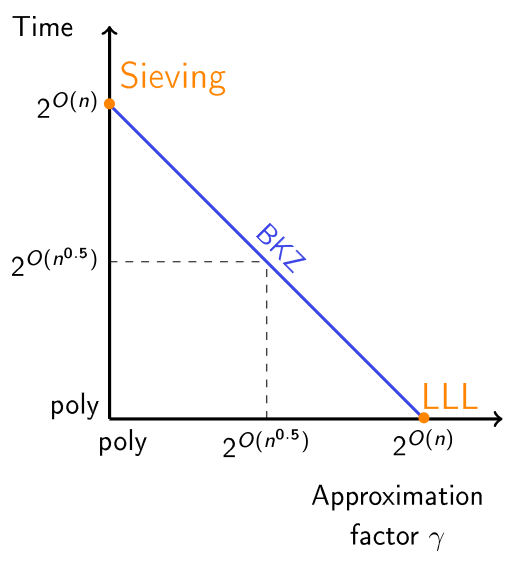
\includegraphics[width=0.4\linewidth]{img/AlicePM_lattices/Screenshot 2025-02-20 at 10-56-37 Lattice reduction algorithms - cryptanalysis.pdf.png}
    \caption{Comparaisons d'algorithmes de réduction de réseau, image proposée par le Dr.Pellet-Mary \cite{AlicePelletMary}}
    \label{fig:SVP_algos}
\end{figure}


\subsection{Signature DSA}\label{DSA}

La sécurité de la signature DSA, Digital Signature Algorithm, repose sur le problème du logarithme discret dans le groupe $\mathbb{Z} / p \mathbb{Z}$ avec $p$ premier et suffisamment grand.

Supposons qu'Alice souhaite signer ses messages. Pour cela, elle doit publier un générateur $g$ d'un sous-groupe de $\mathbb{Z} / p \mathbb{Z}$ d'ordre $q$ un nombre premier (de 160 bits dans la version originale de DSA). Notons qu'il faut alors que $p-1$ admette $q$ comme diviseur. Pour obtenir de tels $p$ et $q$, elle peut suivre les recommandations du NIST \citetitle{dsaFIPS} \cite{dsaFIPS}.
Sa clé secrète est un élément aléatoire $x$ de $\mathbb{Z} / q \mathbb{Z}$, et elle va finalement publier $h=g^{x}$ pour terminer la clé publique qui est donc $(p,q,g,h)$ . \smallbreak
Il est aussi nécessaire d'avoir une fonction $f$ à image dans $\mathbb{Z} / q \mathbb{Z}$. En pratique, on utilise une fonction de hachage. Comme dans le DSA d'origine, nous utilisons SHA-1 pour sa sortie en 160 bits qui peut donc directement être interprété comme un élément de $\mathbb{Z} / q \mathbb{Z}$. \medbreak

Alice a un message $m \in \mathbb{Z} / q \mathbb{Z}$. Pour le signer, elle calcule $b$ tel que :
\begin{empheq}[box={\equations}]{equation}
   m \equiv b y-x f\left(g^{y}\right) \quad(\bmod q) \label{eq:signature}
\end{empheq}

Avec $y \in\{1, \ldots, q-1\}$ aléatoire que l'on appelle clé éphémère. Cette clé, au même titre que la clé privée, doit rester secrète. En revanche, elle peut publier $g^y$ qui ne donne aucune information sur $y$ si le problème du logarithme discret dans $\mathbb{Z} / p \mathbb{Z}$ est bien difficile. Le couple $\left(g^{y}, b\right)$ est la signature de $m$.\medbreak

Pour vérifier la signature, Bob doit vérifier l'égalité suivante :
\begin{empheq}[box={\equations}]{equation*}
   g^{m } \times h^{f(g^{y})}=(g^{y})^b
\end{empheq}

Ce schéma est bien correct dès lors que la signature est bien générée:
\[
g^{m } \times h^{f(g^{y})} = g^{m + xf(g^y)} = g^{yb}
\]


\subsection{Courbes elliptiques et avantage cryptographique}

De même que pour DSA, les courbes elliptiques évoluent dans des groupes modulaires. Ainsi, en prenant $p$ un nombre premier, on peut définir le corps $\mathbb{F}_p$. Puis, on peut construire la courbe elliptique $E$ dans $\mathbb{F}_p$ tel que $\forall x,y \in E$ :

\begin{empheq}[box={\equations}]{equation}
E : y^2 +a_1 xy + a_3 y = x^3 + a_2x^2 + a_4x+a_6\label{eq:EC}
\end{empheq}

Avec $a_1, a_2, a_3, a_4 ,a_6 \in \mathbb{F}_p$ et son discriminant $\Delta$ doit être non nul. Un élément $P$ de $E$ est défini comme un couple ($x,y$), un point de la courbe. Enfin, les opérations élémentaires (addition, soustraction, multiplication et inversion) entre différents éléments de $E$, mettons $P_1$ et $P_2$, sont particulières et peuvent être retrouvées dans le chapitre 3 de notre référence \cite{guide_elliptic_crypto}.\medbreak

Nous souhaitons mettre en évidence la comparaison entre les tailles de clés. Cette comparaison est basée sur le temps nécessaire pour retrouver la clé secrète. Une sécurité de $k$-bits signifie que le meilleur algorithme connu \footnote{Les meilleurs algorithmes connus pour résoudre les problèmes de factorisation d'entier, du logarithme discret et du logarithme des courbes elliptiques sont quantiques. Ils nous permettent de fixer nos critères de sécurité, en revanche on ne sait pas quand les premiers ordinateurs quantiques à usage industriel seront construits.} retrouve la clé privé en $2^k$ étapes. % rho de pollard

\begin{table}[ht]
    \centering
    \caption{Taille de clés pour une sécurité équivalente entre la signature DSA et la signature avec les courbes elliptiques (EC). Issu de \cite{guide_elliptic_crypto}, p.19}
    \begin{tabular}{|lccccc|}
        \toprule
        & \multicolumn{5}{c|}{\textbf{Security level (bits)}} \\
        & 80 & 112 & 128 & 192 & 256 \\
        \midrule
        DSA paramètre $p$  & 1024 & 2048 & 3072 & 8192 & 15360 \\
        EC paramètre $n$ & 160  & 224  & 256  & 384  & 512  \\
        \bottomrule
    \end{tabular}
\end{table}

Ce tableau montre l'avantage d'utiliser les courbes elliptiques. Cette réduction d'un facteur 30 de la taille des paramètres pour un niveau de sécurité de 256 bits rend les courbes elliptiques plus attrayantes pour des implémentations où le support est limité (comme les cartes à puces).

\subsection{Signature ECDSA}

Les courbes elliptiques sont apparues vers le milieu du XIXème siècle \cite{guide_elliptic_crypto}. Elles ont depuis été étudiées pour leur usage à la résolution de nombreux problèmes. Un exemple important est la preuve de la résolution du dernier théorème de Fermat \og$x^n+ y^n = z^n$ n'admet aucune solution entière pour $x,y$ et $z$ si l'entier $n > 2$\fg par Andrew Miles en 1995. C'est en 1985 que Neal Koblitz et Victor Miller firent la première proposition d'utilisation des courbes elliptiques pour un système de chiffrement à clé publique. Nous allons maintenant étudier le protocole de signature qui utilise les courbes elliptiques. \medbreak

Définissons $P$, un point de notre courbe elliptique $E$, d'ordre un nombre premier $n$, soit $H : \{0, 1\}^* \to \{1, \dots, n - 1\}$ notre fonction de hachage. La fonction SHA-512 est souvent utilisée avec une troncature de sortie pour obtenir $\ell$ bits, où $\ell$ est le nombre de bits de $n$. \smallbreak

Nous définissons notre clé secrète $x \in \mathbb{N^*_n}$ et notre clé publique $Q = xP$. La signature d'un message $m$ avec la clé $x$ implique de choisir une clé éphémère aléatoire $r \in \mathbb{N^*_n}$ et de calculer $R = (x_R, y_R) = rP$. Si $x_R \mod n = 0$, une autre valeur de $r$ est choisie. La signature est alors donnée par $\sigma = (\sigma_1, \sigma_2) = (x_R \mod n, s)$, où :
\[
s \equiv r^{-1}(x(x_R \mod n) + H(m)) \pmod{n}.
\]
Si $s \equiv 0 \mod n$, une autre valeur de $r$ est choisie.

Pour vérifier une signature $(\sigma_1, \sigma_2)$, on vérifie que $Q$ appartient à la courbe, qu'il est d'ordre $n$, et que $1 < \sigma_i < n$ pour $i = 1,2$. On calcule ensuite les valeurs :
\[
u_1 \equiv H(m) \sigma_2^{-1} \pmod{n}, \quad u_2 \equiv \sigma_1 \sigma_2^{-1} \pmod{n}.
\]
Enfin, on détermine le point $(x_1, y_1) = u_1 P + u_2 Q$. La signature est valide si $\sigma_1 \equiv x_1 \pmod{n}$.

La vérification de la signature se fait grâce à :
\[
\begin{aligned}
    u_1 P + u_2 Q &= (u_1 + u_2 x) P \\
                  &= (H(m) s^{-1} + (x_R \mod n) s^{-1} x) P \\
                  &= s^{-1} (H(m) + (x_R \mod n) x) P \\
                  &= r (H(m) + x(x_R \mod n))^{-1} (H(m) + (x_R \mod n) x) P \\
                  &= rP.
\end{aligned}
\]

ECDSA est un protocole de signature largement utilisé, implémenté dans diverses bibliothèques telles qu'OpenSSL, et couramment employé dans les cryptomonnaies comme Bitcoin ou Ethereum.


\section{Attaque par canal auxiliaire} \label{sec:attaque_canal}

\subsection{Description rapide}

Les attaques par canal auxiliaire consistent principalement à exploiter des failles matérielles ou logicielles pour récupérer de l'information sur les données manipulées lors de l’exécution d'un algorithme. Ainsi, un protocole peut quand même être compromis malgré sa robustesse mathématique. Par exemple, en mesurant la consommation de courant de l'appareil attaqué, il est possible de récupérer de l'information sur les opérations effectuées par son processeur et même de récupérer des bits de clé. Il est aussi possible d'exploiter le temps d’exécution, les émissions électromagnétiques ou même sonores du processeur.\medbreak

Il existe également des attaques plus invasives/destructrices comme celles par injections de fautes pour étudier ensuite le comportement du processeur. Enfin, la plus radicale mais également la plus coûteuse consiste à ajouter une sonde directement sur le circuit pour mesurer les bits transitant par le bus sondé.\medbreak

Nous appellerons "trace" la mesure obtenue lors d'une attaque par canal auxiliaire. En pratique, les traces sont soumises à des bruits et des imprécisions de mesure qui peuvent masquer l'information voulue. Cela mène nécessairement à des erreurs lors de leurs traitements. Dans notre cas, nous supposons de manière assez simpliste, avoir à notre disposition des traces parfaites, non bruitées mais partielles des éléments privés. C'est-à-dire que nous connaissons avec certitude une certaine proportion de bits de ce qui nous intéresse.


\subsection{Illustration d'une trace}

 Appelons $x$ la valeur dont on veut récupérer les bits d'informations, admettons par exemple que $x$ s'écrit ainsi :

\begin{center}
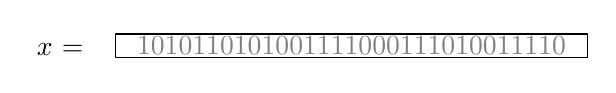
\begin{tikzpicture}
    \draw (0,0) rectangle (6,0.3) ;
    \draw (-0.7,0.1) node {$x$ =};
    \draw (3,0.15) node[gray] {1010110101001111000111010011110};

\end{tikzpicture}
\end{center}

L'information inconnue de $x$, en rouge sur les schémas ci-dessous, peut être organisée de différentes manières. La plus simple étant le cas contigu où juste un bloc de bits est manquant :\smallbreak


\begin{enumerate}
  \item[Cas contigu :]
    \begin{center}
        %left
        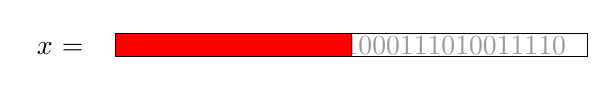
\begin{tikzpicture}
            \draw (0,0) rectangle (6,0.3);
            \draw (-0.7,0.1) node {$x$ =};
            \draw (3,0.14) node[gray!80] {1010110101001111000111010011110};
            \filldraw[fill=red] (0,0) rectangle (3,0.3);
        \end{tikzpicture}
        \smallbreak

        %right
        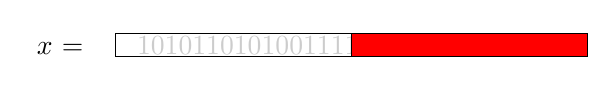
\begin{tikzpicture}
            \draw (0,0) rectangle (6,0.3);
            \draw (-0.7,0.1) node {$x$ =};
            \draw (3,0.14) node[gray!40] {1010110101001111000111010011110};
            \filldraw[fill=red] (3,0) rectangle (6,0.3);
        \end{tikzpicture}
        \smallbreak

        %center
        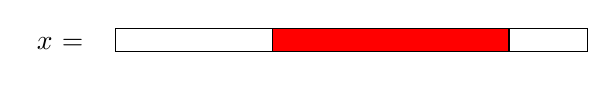
\begin{tikzpicture}
            \draw (0,0) rectangle (6,0.3);
            \draw (-0.7,0.1) node {$x$ =};
            \filldraw[fill=red] (2,0) rectangle (5,0.3);
        \end{tikzpicture}
        \smallbreak
   \end{center}
\end{enumerate}

Mais nous prenons aussi en compte le cas où l'information manquante est séparée en plusieurs blocs :

\begin{enumerate}
   \item[Cas non-contigu :]
   \begin{center}
        %non contigous
        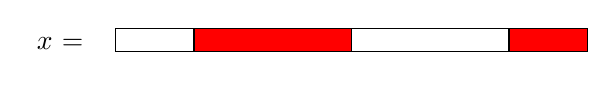
\begin{tikzpicture}
            \draw (0,0) rectangle (6,0.3);
            \draw (-0.7,0.1) node {$x$ =};
            \filldraw[fill=red] (1,0) rectangle (3,0.3);
            \filldraw[fill=red] (5,0) rectangle (6,0.3);
        \end{tikzpicture}
        \smallbreak

        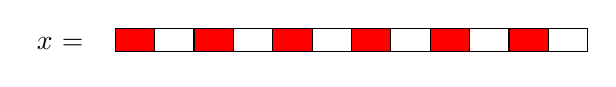
\begin{tikzpicture}
            \draw (0,0) rectangle (6,0.3);
            \draw (-0.7,0.1) node {$x$ =};
            \foreach \k in {0.5, 1.5, ..., 6}
                {\filldraw[fill=red] (\k - 0.5,0) rectangle (\k,0.3);}

        \end{tikzpicture}
        \smallbreak
        
        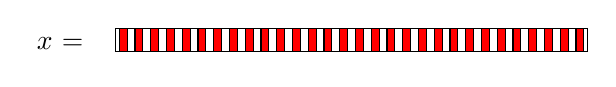
\begin{tikzpicture}
            \draw (0,0) rectangle (6,0.3);
            \draw (-0.7,0.1) node {$x$ =};
            \foreach \k in {0.15, 0.35, ..., 6.05}
                {\filldraw[fill=red] (\k - 0.1,0) rectangle (\k,0.3);}

        \end{tikzpicture}
    \end{center}
\end{enumerate}

\bigskip

Cette différence est à prendre en compte lors de la représentation mathématique des données et de la mise en équation. En l’occurrence, pour une même proportion $\epsilon$ de bits de $x$ \textbf{connus} (partie blanche de nos schémas), la taille de notre réseau augmente linéairement avec le nombre de blocs inconnus.




% -------------------------------------------------------------------------------
%
%  DSA et attaque
%
% -------------------------------------------------------------------------------


\newpage
\section{Attaque par réduction de réseau} \label{sec:attaque_signature}

L'attaque que nous étudions est celle de Howgrave-Graham et Smart publiée en 1999 \cite{latAtk}. Nous en représentons les bases mathématiques et son application.

\subsection{Stratégie de l'attaque}\label{Stratégie de l'attaque}


Comme nous l'avons précisé plus tôt, l'attaque nécessite l'utilisation de canaux auxiliaires pour récupérer des bits d'information. En l'occurrence, il nous faut de l'information sur les clés éphémères $y_i$ utilisées lors de plusieurs signatures et éventuellement de l'information sur la clé privée $x$ directement. Cette dernière n'est en effet pas obligatoire, elle peut être compensée par une signature supplémentaire.
L'objectif est de retrouver entièrement une clé éphémère et d'en déduire $x$ à l'aide de l'équation \ref{eq:signature}. \smallbreak

Admettons que l'on puisse récupérer $h$ signatures, alors en utilisant notre équation \ref{eq:signature}, on peut construire $h$ équations pour $1\leq i \leq h$:

\begin{empheq}[box={\equations}]{equation}
   m_{i} - b_{i} y_{i} + x f\left(g^{y_{i}}\right) \equiv 0\quad(\bmod q)
\end{empheq}
\smallbreak

On peut ensuite réarranger nos équations, avec $A$ et $B$ entiers, sous cette forme $y_{i} + x \times A_{i} + B_{i} \equiv 0\quad(\bmod  q)$.
Avec un pivot de Gauss utilisant une équation de notre choix (ici on choisit la dernière équation $i=h$) on peut exprimer $x$ en fonction de $y_h$. Nos équations sont alors de la forme :
\begin{empheq}[box={\equations}]{equation}
   y_{i} + y_{h} \times A^{\prime}_{i} + B^{\prime}_{i} \equiv 0 \quad(\bmod q)\label{eq:milieu}
\end{empheq}


Nous allons enfin exploiter la connaissance que nous avons des $y_{i}$. Nous nous plaçons dans un premier temps dans le cas contigu où l'information manquante est un seul bloc de bits, avec cette représentation :

\begin{center}
    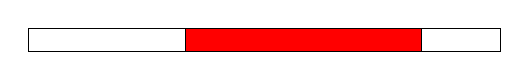
\begin{tikzpicture}
            \draw (0,0) rectangle (6,0.3);
            \filldraw[fill=red] (2,0) rectangle (5,0.3);
        \end{tikzpicture}
\end{center}

Cette connaissance peut alors être exprimée ainsi:

\begin{empheq}[box={\equations}]{equation}
y_{i}=\alpha_{i}^{\prime}+2^{\lambda_{i}} z_{i}+2^{\mu_{i}} \alpha_{i}^{\prime \prime}\label{eq:cle_y}
\end{empheq}

On connaît les $\alpha_{i}^{\prime}$, $\alpha_{i}^{\prime \prime}$, $\lambda_{i}$ et $\mu_{i}$. Nos inconnues sont les $z_{i}$ et on défini $X_i$ leurs bornes supérieures  :

$$
0 \leq z_{i}^{\prime}<2^{\lambda_{i}}, 0 \leq z_{i}<X_{i}=2^{\mu_{i}-\lambda_{i}}, \lambda_{i}<\mu_{i} \text { and } 0 \leq z_{i}^{\prime \prime}
$$

On simplifie une dernière fois nos équations pour obtenir :
\begin{empheq}[box={\equations}]{equation}
  z_{i}+s_{i} z_{h}+t_{i} = 0 \quad(\bmod q)  
\end{empheq}

De tels systèmes d'équations devraient avoir des solutions avec $z_i \approx q$. L'heuristique principale de cette attaque revient à dire que les petites solutions comme celle dont on connaît l'existence ($z_i < X_i < q$) sont rares. Rare à un point où il suffit d'en trouver assez petite pour considérer que c'est bien celle que l'on cherche.
Nous allons maintenant étudier comment il nous est possible de trouver une solution bornée par les $X_i$ à ce système de $n = h-1$ équations modulaires.

\smallbreak
Le développement complet entre ces différentes équations est consultable en annexe \ref{annexe:Developpement}.



\subsection{Construction de l'instance CVP}

Pour cela, nous allons utiliser un réseau euclidien en construisant la matrice $A$ :

$$
A=\left(\begin{array}{ccccc}
-1 & s_{1} & s_{2} & \ldots & s_{n} \\
0 & q & 0 & \cdots & 0 \\
0 & 0 & q & & 0 \\
\vdots & & & \ddots & \vdots \\
0 & \cdots & \cdots & \cdots & q
\end{array}\right) \in M_{(n+1),(n+1)}(\mathbb{Z})
$$

On s'intéresse donc au réseau $L=\left\{\mathbf{x} A: \mathbf{x} \in \mathbb{Z}^{n+1}\right\}$ issu de $A$. 
En développant, un vecteur $\mathbf{v}$ de $L$ s'exprime ainsi :
$$
\mathbf{v} = (-x_0 ,\, x_0s_1 + x_1q, \, \ldots, \, x_0s_n +x_nq)\in \mathbb{Z}^{n+1}
$$

On rappelle que l'équation (5) donne $z_i \equiv -z_hs_i - t_i \mod q $.
Ainsi, en prenant le vecteur cible $\mathbf{t}$ suivant :
$$
\mathbf{t}=\left(0, t_{1}, t_{2}, \ldots, t_{n}\right) \in \mathbb{Z}^{n+1}
$$

On sait par construction qu'il existe un vecteur $\mathbf{v}$ de $L$ qui donne :
$$
\mathbf{v} - \mathbf{t} = (z_0,\, z_1,\, \ldots,\, z_n) \in \mathbb{Z}^{n+1}
$$

et dont la distance à $\mathbf{t}$ est bornée par :
$$
\Vert \mathbf{v} - \mathbf{t} \Vert^2 \leq \sum_{i=0}^{n} X_i^2
$$ 


Ainsi, on espère qu'après la réduction du réseau, Babaï puisse respecter cette borne et retourner $\mathbf{v} \in L$  pour que $\mathbf{v} - \mathbf{t}$ soit la réponse à notre problème.\medbreak
Howgrave-Graham et Smart estiment que si LLL fonctionne mieux qu'en théorie (ce qui est le cas en pratique pour des valeurs de $n$ pas trop grandes) la condition suivante est suffisante pour que Babaï fonctionne :

$$
\max\limits_{0 \leq i \leq n} X_i < q^{n/(n+1)}
$$ 

En notant que les $X_i = q^{1-\epsilon}$ on a 
$$
q^{1-\epsilon} < q^{n/(n+1)}
$$
D'où :
$$
\epsilon > \frac{1}{n+1}
$$
Donc, plus on a de traces de clé éphémères de signatures, plus le nombre de bits connus nécessaire est petit.

 Ils pensaient également que si Babaï retourne un vecteur différent de la solution voulue,il pourrait quand même être suffisamment proche de $\mathbf{t}$. On pourrait ainsi obtenir des clés éphémères "boguées" qui permettraient à l'attaquant de se faire passer pour le signataire en les révélant. Ceci dit, nous ne sommes pas parvenu à trouver de telles clés.




\subsection{Cas non-contigu}

Passons maintenant au cas où les traces de nos clés éphémères peuvent avoir plusieurs blocs inconnus :

\begin{center}
    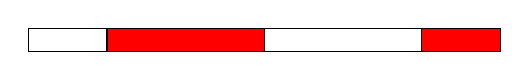
\begin{tikzpicture}
        \draw (0,0) rectangle (6,0.3);
        \filldraw[fill=red] (1,0) rectangle (3,0.3);
        \filldraw[fill=red] (5,0) rectangle (6,0.3);
    \end{tikzpicture}
\end{center}

On peut les exprimer ainsi :
$$
y_i = z'_i + \sum_{j=0}^{d}z_{i,j}2^{\lambda_{i,j}}
$$

Avec $z_{i,j}$ des inconnues de bornes $Z_{i,j}$ :
$$
z_{i,j} < Z_{i,j} < 2^{\lambda_{i,j+1}-\lambda_{i,j}}
$$

On part aussi du principe que cette quantité de bits inconnus est approximativement la même pour tout $i$ :
$$\prod_{j=1}^{d} Z_{i, j} \approx q^{1-\epsilon}$$

En remplaçant les $y_i$ dans les équations du système (3), on obtient après simplification :
\begin{empheq}[box={\equations}]{equation}
z_{i, 1}+\sum_{j=2}^{d} s_{i, j} z_{i, j}+\sum_{j=1}^{d} r_{i, j} z_{0, j}+t_{i} \equiv 0 \quad(\bmod q) 
\end{empheq}

avec les $s_{i,j}$, $r_{i,j}$ et $t_i$ dans $\mathbb{Z} / q \mathbb{Z}$ \smallbreak

La matrice génératrice du réseau de taille $d(n+1)$ est construite ainsi :
$$
A=\left(\begin{array}{c|c}
-I_{d(n+1)-n} & R^{t} \\
& S \\
\hline 0 & -q I_{n}
\end{array}\right) \times D
$$

Où $R=\left(r_{i, j}\right)$ et $S$ correspond à la matrice

$$
S=\left(\begin{array}{ccc}
\mathbf{s}_{1} & & 0 \\
& \ddots & \\
0 & & \mathbf{s}_{n}
\end{array}\right) \in M_{n(d-1), n}(\mathbb{Z})
$$

avec $\mathbf{s}_{i}$ le vecteur colonne $\left(s_{i, j}\right)_{j=2}^{d}$.\smallbreak


La matrice $D$ est là pour pondérer notre réseau afin de prendre en compte les variations de taille des $Z_{i,j}$. C'est la matrice diagonale suivante :

$$
\begin{aligned}
D & =\operatorname{diag}\left(J_{0,1}, \ldots, J_{0, d}, J_{1,2}, \ldots, J_{1, d}, \ldots, J_{n, 2}, \ldots, J_{n, d}, J_{1,1}, \ldots, J_{n, 1}\right) \\
& =\operatorname{diag}(\mathbf{j})
\end{aligned}
$$

Avec $J_{i, j}=J / Z_{i, j} \in \mathbb{Z}$ pour $J=\prod_{\substack{0 \leq i \leq n \\ 1 \leq j \leq d}} Z_{i, j} \simeq q^{(1-\epsilon)(n+1)}$

Le vecteur cible est $\mathbf{t}=\left(0, \ldots, 0, t_{1} J_{1,1}, \ldots, t_{n} J_{n, 1}\right)$ où seules les $n$ dernières coordonnées sont non-nulles, et pondérées.

Par construction, on sait l'existence d'un vecteur $\mathbf{v}$ de $L$ tel que :
$$
\mathbf{v} B-\mathbf{t}=\left(z_{0,1}, \ldots, z_{0, d}, z_{1,2}, \ldots, z_{1, d}, \ldots, z_{n, 2}, \ldots, z_{n, d}, z_{1,1}, \ldots, z_{n, 1}\right) \cdot \mathbf{j}
$$
Comme en version contiguë, on espère que le vecteur retourné par Babai soit le bon $\mathbf{v}$.



% -------------------------------------------------------------------------------
%
%  ECDSA et attaque
%
% -------------------------------------------------------------------------------


\newpage
\section{Résultats} \label{sec:résultats}

\subsection{Résultats du cas contigu}

Nous réalisons cette attaque en considérant que nous pouvons récupérer des traces de longueur choisie et sans erreur. Ces conditions sont très fortes, ainsi mesurer le temps total d'une attaque réelle est difficile. Cela dépend de la capacité des attaquants à récupérer de l'information pendant l'exécution du système cible et de la qualité des traces récupérées. Nous ne faisons aucune hypothèse sur la manière de récupérer et de traiter les données nécessaires aux attaques. Par conséquent, nous n'intégrons pas le temps nécessaire à la récupération des signatures et à l'analyse de leurs traces dans nos expériences. \smallbreak

Pour former les traces de l'équation (4), on utilise une fonction qui retourne un $\lambda$ aléatoire $\mu = \lambda + floor(\epsilon\times size(q))$ qui délimitent le bloc de bits à enlever.
De même, on considère que les étapes de reformulation d'équations et de construction de matrice peuvent se faire durant la phase de récupération des traces. On va donc considérer ici uniquement le temps de résolution de CVP. Nous présentons ci-dessous la structure de notre implémentation :

\begin{algorithm}
\caption{\citetitle{latAtk}}
\begin{algorithmic}[1]
\Require $nb\_signature, epsilon, Zq, g, x$  \Comment{Paramètres pour la génération des signatures}
\State $\beta = generate\_signature(nb\_signature, epsilon, Zq, g, x)$
\State $eq = create\_equation(\beta)$
\State $A = matrix\_from\_equations(eq)$
\State $Z = plus\_court\_vecteur(A)$ \Comment{Opération chronométrée}
\Ensure $verification(\beta,Z)$

\end{algorithmic}
\end{algorithm}

\medbreak

La programmation a été réalisée en \textit{Python} grâce à la librairie \textit{SageMath}. Nous avons utilisé les mêmes fonctions que celles indiquées dans l'article de référence \cite{latAtk}. Nous pouvons voir dans le tableau \ref{tab:comparaison_signatures} les résultats publiés au regard de ce qu'il est aujourd'hui possible de réaliser.

\begin{center}
    \begin{table}[H]
        \centering
        \caption{Comparaison de résultats entre \cite{latAtk} et notre implémentation, temps évalué sur l'ordinateur \ref{bergman} }
        \label{tab:comparaison_signatures}
        
        \begin{tabular}{|c|c|cc|cc|}
            \toprule
            Epsilon & Bits connus & \multicolumn{2}{|c|}{Nombre d'équations\footnote{Le nombre d'équations présenté est le minimum requis pour que l'attaque fonctionne.}} & \multicolumn{2}{|c|}{Temps (secondes)} \\
            \cmidrule{3-6}
            && Nous & Eux & Nous & Eux \\
            \midrule
                0.5   & 80 & 2  & 2  & 0.00303  & 0.0102  \\
                0.25  & 40 & 4  & 4  & 0.00428  & 0.0360 \\
                0.1   & 16 & 10 & 11 & 0.00956  & 0.4428 \\
                0.05  & 8  & 24 & 30 & 0.05998 & 8.6970 \\
                0.03125 & 5  & 80 & $/$  & 7163.72 & \textit{échec} \\
                % 0.025 & 4 & \textit{to determine} & - & \textit{A calculer} & - \\
            \bottomrule
        \end{tabular}
    \end{table}
\end{center}

% TODO 14h50 test avec n=80 e=0.025, p=1024 et q=160,
% sage src/main.sage 80 0.035 test t

% sur plomet: 17h24 (2h30) - DSA99 attack :
%actual_z1: 0x2aa51af1e72951f1c4be03c9750e0e5cfe3b26c43d835808ef16ccd1
%hidden_z1: 0x20000000000000000000000000000000000000000000000000000001
%z1_found : 0x2aa51af1e72951f1c4be03c9750e0e5cfe3b26c43d835808ef16ccd1
%z1_found == actual_z1:  True
%Attack duration : 7163.722145318985


La différence entre leurs temps d'exécution et les nôtres repose grandement sur l'évolution technologique depuis 2001, cf. les configurations des machines \ref{annexe:machines} utilisées pour l'attaque. Le(s) processeur(s) utilisé(s) pour réaliser leurs attaques en 1999 ne sont pas indiqués dans leur article.\medbreak

Lors de nos expériences, nous avons vu que la RAM utilisée par notre processus lors de nos tests était inférieure à 2 Gigaoctets. On considère que la mémoire est peu optimisée en Sage, l'espace mémoire utilisé pour faire la réduction de réseau est une petite fraction de ce total.
 
On estime que la capacité de leur RAM était comprise entre 128 et 512 Mégaoctets, vous pourrez trouver plus de détails dans le tableau \ref{tab:ddr_comparaison} en annexe.


\medbreak

Cette expérience montre la pertinence de l'évolution des protocoles de sécurité. Face à ce type d'attaque, DSA présente peu de résistance. Nous verrons par la suite si l'augmentation de la taille des paramètres ou le changement de la fonction de hachage permet de renforcer la signature.


\subsection{Résultats du cas non-contigu}

Dans leur papier, le nombre de blocs inconnus $d$ est toujours une puissance de 2. Cela est sûrement dû à la fonction qu'ils ont utilisée pour générer leurs $z'_i$ et $\lambda_{i,j}$. Pour simplifier le code, notre implémentation vient aussi avec ses limitations. On prend $d$ qui divise le nombre de bits de $q$ et les blocs de bits effacés font tous la même taille : $(1-\epsilon)\times\frac{size(q)}{d}$ \smallbreak
Nos valeurs sont des moyennes sur 100 exécutions sur l'ordinateur \ref{lautrec}, nous indiquons la probabilité de réussite entre parenthèse lorsque celle-ci n'est pas de 100\%.

\begin{center}
    \begin{table}[H]
        \centering
        \caption{Comparaison de résultats entre \cite{latAtk} et notre implémentation}
        \label{tab:comparaison_signatures_non_contigu}
        
        \begin{tabular}{|c|c|cc|cc|}
            \toprule
            Epsilon & $d$  & \multicolumn{2}{|c|}{Nombre d'équations} & \multicolumn{2}{|c|}{Temps (secondes)} \\
            \cmidrule{3-6}
            && Nous & Eux & Nous & Eux \\
            \midrule
                0.5 & 2  & 2 & 2 & 0.0026 & 0.067  \\
                    & 4  & 2 & 2 & 0.0067 & 0.304  \\
                    & 8  & 2 & 2 & 0.032 & 1.135 \\
                    & 16 & 3 {\footnotesize (6\%)} & $/$ & 0.899 & \textit{échec} \\
                \hline
                0.25 & 2 & 4 & 4 & 0.050 & 0.393 \\
                     & 4 & 4 {\footnotesize (95\%)} & 4 & 0.024 & 1.785 \\
                     & 8 & 5 {\footnotesize (3\%)} & $/$ & 0.452 & \textit{échec} \\
                \hline
                 0.1 & 2 & 12 {\footnotesize (88\%)} & 12 & 0.087 & 6.256 \\
                     & 4 & $/$ & $/$ & \textit{échec} & \textit{échec} \\
                \hline
                0.05 & 2 & $/$ & 20 & \textit{échec} & \textit{échec} \\
    
            \bottomrule
        \end{tabular}
    \end{table}
\end{center}



\subsection{Remarque}

\begin{center}
    \begin{table}[H]
        \centering
        \caption{Extrait de résultat sur DSA historique, non contigu sur \ref{lautrec}, contigu sur \ref{plomet}}
        \label{tab:echec_non_contigu}
        \begin{tabular}{|c|c|c|c|c|}
            \toprule
            & Epsilon & Nombre d'équations & Temps (secondes) & Réussite \\
            \midrule
             Non Contigu (d=16) \label{tab:obsrv1} &  0.4     & 6  & 142.297 & \textit{False} \\
             Contigu \label{tab:obsrv2}    &  0.03125 & 80 & 7163.72 & \textit{True} \\
            \bottomrule
        \end{tabular}
    \end{table}
\end{center}

Dans ce tableau, on remarque qu'il est possible de faire fonctionner l'attaque avec seulement 5 bits de connaissances sur chacune des 80 traces dans le cas contigu. Alors qu'avec 40\% des bits connus, c'est à dire 64 bits de connaissances en non-contigu, nous ne parvenons pas à faire fonctionner l'attaque lorsqu'ils sont séparés en trop de blocs.

\medbreak

Il serait alors peut être plus intéressant de ne considérer que les bits que l'on connaît sur les extrémités de la trace afin de ne considérer que le cas contigu :

\medbreak
\begin{center}
    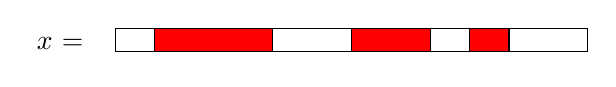
\begin{tikzpicture}
        \draw (0,0) rectangle (6,0.3);
        \draw (-0.7,0.1) node {$x$ =};
        \filldraw[fill=red] (0.5,0) rectangle (2,0.3);
        \filldraw[fill=red] (3,0) rectangle (4,0.3);
        \filldraw[fill=red] (4.5,0) rectangle (5,0.3);
    \end{tikzpicture}
    \smallbreak
    \begin{tikzpicture}[overlay]
        \draw[->, line width=2pt] (0.5,0.5) -- (0.5,0);
    \end{tikzpicture}
    \smallbreak
    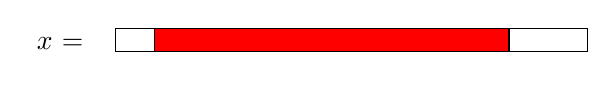
\begin{tikzpicture}
        \draw (0,0) rectangle (6,0.3);
        \draw (-0.7,0.1) node {$x$ =};
        \filldraw[fill=red] (0.5,0) rectangle (5,0.3);
    \end{tikzpicture}
\end{center}


Dans le cas de notre implémentation, quitte à augmenter le nombres de traces nécessaires, il faudrait $\epsilon' > 0.03$ si l'on note $\epsilon'$ la proportion de bits connus sur les bords de nos traces du cas non-contigu.




\subsection{Résultats pour ECDSA}


La signature que l'on attaque dans la suite de ce document est portée sur une courbe elliptique recommandée par le NIST : \textbf{P-256}. Son implémentation suit les instructions détaillées dans ce document : \citetitle{NIST_ECDSA}\cite{NIST_ECDSA}.

\smallbreak

L'attaque que l'on réalise est la même que celle décrite en section \ref{Stratégie de l'attaque}. La récupération de l'information et son évaluation sont identiques. Les calculs présentés ci-dessous ont été réalisés sur l'ordinateur \ref{jolicoeur}. Il y a (seulement) 5 répétitions pour chaque valeur de epsilon, la valeur présentée en temps est une moyenne, et le nombre de signatures est la plus grande valeur requise pour que la récupération de la clé privée fonctionne.

% Jeu de données : contigu/P-256/jolicoeur_2025_02_04_10_52

\begin{center}
    \begin{table}[ht]
        \centering
        \caption{Évaluation de l'attaque sur ECDSA P-256 avec l'algorithme LLL en fonction du pourcentage de connaissance des clés éphémères $\epsilon$ }
        \label{tab:attaque_ECDSA}
        
        \begin{tabular}{|c|c|c|}
            \toprule
            $\epsilon$ & Nombre de signatures & Temps (seconde) \\
            \midrule
            0.05 &                   26 &         0.71274    \\
            0.1  &                   11 &         0.125615   \\
            0.15 &                    8 &         0.058946   \\
            0.2  &                    6 &         0.0459488  \\
            0.25 &                    5 &         0.0379201  \\
            0.3  &                    4 &         0.0276537  \\
            0.35 &                    3 &         0.0173285  \\
            0.4  &                    3 &         0.0172096  \\
            0.45 &                    3 &         0.0199899  \\
            0.5  &                    3 &         0.0138443  \\
            \bottomrule
        \end{tabular}
    \end{table}
\end{center}

% -------------------------------------------------------------------------------
%
%  Etude concrète approfondie
%
% -------------------------------------------------------------------------------

\newpage

\section{Tests d'algorithmes et paramètres} \label{sec:epreuves}

\subsection{Expériences avec DSA}

Nous avons testé cette attaque sur DSA en augmentant la taille des paramètres, en section \ref{sec:preambule} avec le tableau \ref{tab:comparaison_signatures} on a évalué pour $q$ de 160 bits. Nous allons voir ici pour $q$ de 224 et 256. Nous avons porté nos choix de taille de $q$ sur ces valeurs car ce sont celles qui sont recommandés par différentes agences nationales \cite{NIST_ECDSA}.\smallbreak
Nous avons pu tester différents algorithmes de réduction pour observer leurs performances associées, LLL, BKZ de la librairie \textit{Sagemath} et BKZ de la librairie \textit{NTL} \cite{NTL}. Le second BKZ est nommé \textbf{BKZ2} dans la suite de ce rapport.\smallbreak

Dans le cadre de BKZ, un paramètre supplémentaire intervient, la taille $\beta$ des blocs, dans cette section, $\beta$ est fixée à 10. 

Nous pouvions faire des test en modifiant le mode de l'attaque (contigu ou non), la proportion de connaissance de la clé (nommé epsilon), l'algorithme de réduction de réseau et l'algorithme pour trouver le point le plus proche du réseau. Nous avons essayé de couvrir le plus de combinaisons possibles.\smallbreak

%Nous avons testé LLL et ses variantes comme fpLLL avec différentes représentation mémoire des éléments.
%Nous avons aussi essayé BKZ basé sur fpLLL ou sur NTL en faisant varier la taille des blocs.


Nous avons eu des difficultés pour récupérer la clé privée à l'issue de l'attaque quand la connaissance des clés éphémères était inférieure ou égale à 5 bits. 

\begin{table}[H]
    \centering
    \caption{Nombre de bits connus (arrondis à l'entier inférieur) en fonction de la valeur de epsilon et de la taille du groupe utilisé}
    \begin{tabular}{|c|c|c|c|c|}
        \toprule
        Epsilon & 160 & 224 & 256 & 320\\
        \midrule
        0.02 & 3 & 4 & 5 & 6 \\
        0.025 & 4 & 5 & 6 & 8 \\
        0.03 & 4 & 6 & 7 & 9 \\
        0.035 & 5 & 7 & 8 & 10 \\
        0.04 & 6 & 8 & 10 & 12 \\
        \bottomrule
    \end{tabular}
    \label{tab:epsilon_bits}
\end{table}

Nous allons faire une légère aparté pour apporter plus de précision sur la collecte des données que l'on a effectué.\medbreak

Chaque expérience était défini selon l'algorithme de réduction employé, les valeurs minimales et maximales de epsilon et les paramètres de la signature. Puis nous écrivions dans notre base de données le nombre minimale de signature nécessaire, et le temps associé, pour que l'attaque aboutisse sur la valeur d'epsilon testé. À chaque itération, nous générions les traces nécessaires pour l'attaque.

\newpage
\subsubsection{DSA contigu}

Voici trois graphes que l'on peut observer, avec des données évaluées sur \ref{perbosc}.

\begin{figure}[H]
    \centering
    \begin{minipage}{0.45\textwidth}
        \centering
        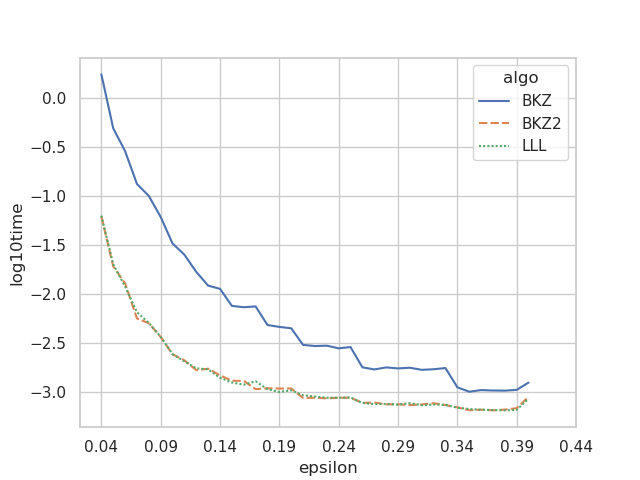
\includegraphics[width=\textwidth]{img/contigu/1024_160_mint_maxm_epsi_time_log.png}
        \caption{1024 160}
        \label{fig:1024 160}
    \end{minipage}
    \hfill
    \begin{minipage}{0.45\textwidth}
        \centering
        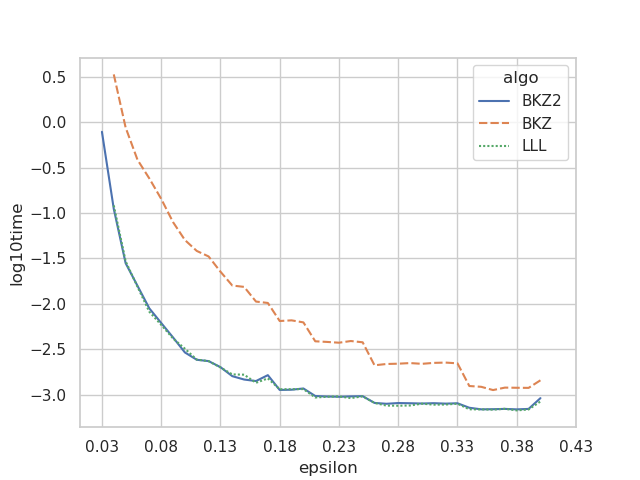
\includegraphics[width=\textwidth]{img/contigu/2048_224_mint_maxm_epsi_time_log.png}
        \caption{2048 224}
        \label{fig:image2}
    \end{minipage}
    \vfill
    \begin{minipage}{0.45\textwidth}
        \centering
        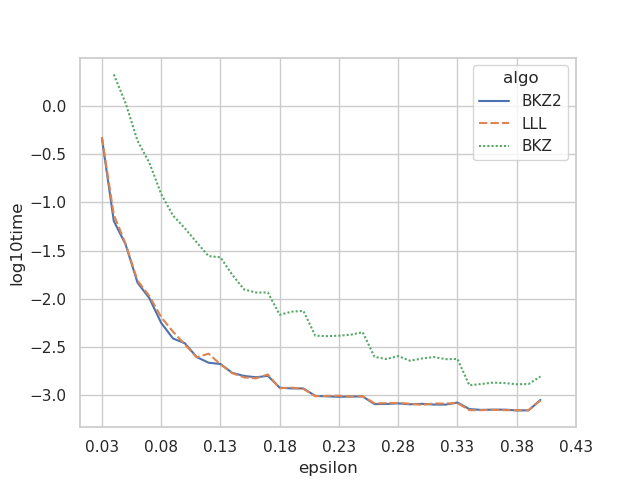
\includegraphics[width=\textwidth]{img/contigu/3072_256_mint_maxm_epsi_time_log.png}
        \caption{3072 256}
        \label{fig:image3}
    \end{minipage}
    \caption{Graphes couvrant les différents $p$, $q$ reconnus par le NIST}
    \label{fig:contigu}
\end{figure}

Peu importe les paramètres des courbes, on remarque que BKZ est plus lent que LLL, ce qui est prévu par la théorie. En revanche, l'implémentation de Victor Shoup \cite{NTL} semble aussi performante que LLL.\smallbreak
D'autres part, le nombre de messages nécessaires pour réussir l'attaque est très proche pour les trois algorithmes.
Avec des valeurs de epsilon plus faible, et donc un réseau plus grand, on s'attendrait à voir émerger un avantage pour BKZ avec des blocs de taille 10. En effet, le facteur d'approximation s'améliore quand la taille des blocs grandit comme représenté dans la figure \ref{fig:SVP_algos}.

%%%%%%%%%%%%%%%%%%%%%%%%%%%%%%%%%%%%%%%%%%%%
%%%%%%%%%%%%%%%%%%%%%%%%%%%%%%%%%%%%%%%%%%%%
%%%%%%%%%%%%%%%%%%%%%%%%%%%%%%%%%%%%%%%%%%%%
% section non contigu
\newpage
\subsubsection{DSA non-contigu}

De même que la section précédente, nous avons obtenu ces données sur \ref{perbosc}. Elles ont été tracés avec $d$ de taille 2.

\begin{figure}[H]
    \centering
    \begin{minipage}{0.45\textwidth}
        \centering
        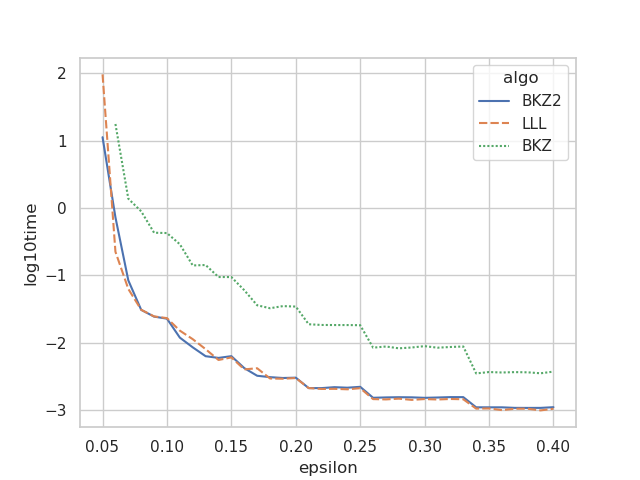
\includegraphics[width=\textwidth]{img/non_contigu/1024_160_mint_maxm_epsi_time_log.png}
        \caption{1024 160}
        \label{fig:1024 160_non_contigu}
    \end{minipage}
    \hfill
    \begin{minipage}{0.45\textwidth}
        \centering
        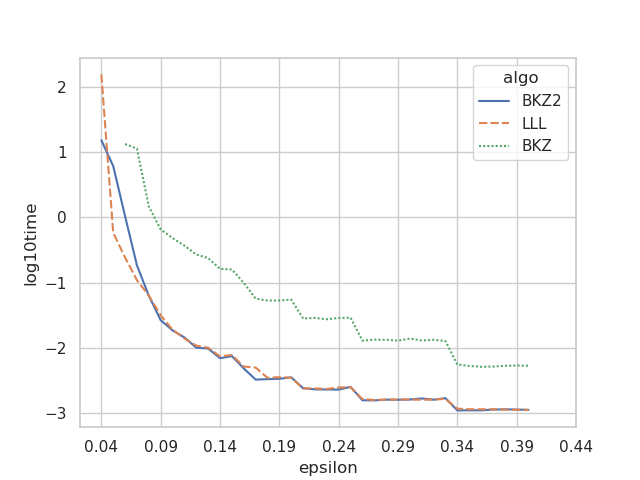
\includegraphics[width=\textwidth]{img/non_contigu/2048_224_mint_maxm_epsi_time_log.png}
        \caption{2048 224}
        \label{fig:image2_non_contigu}
    \end{minipage}
    \vfill
    \begin{minipage}{0.45\textwidth}
        \centering
        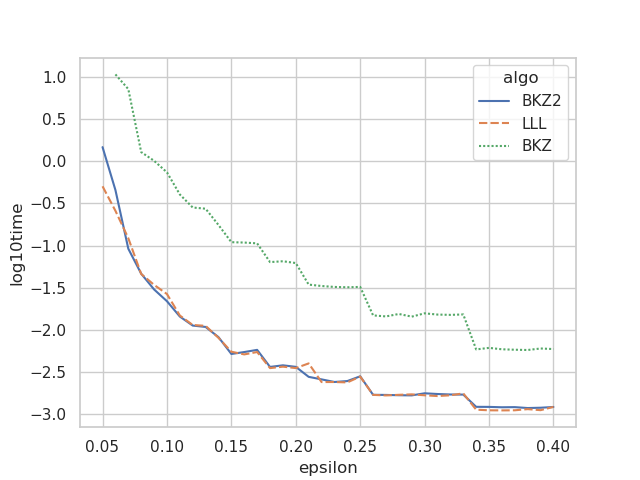
\includegraphics[width=\textwidth]{img/non_contigu/3072_256_mint_maxm_epsi_time_log.png}
        \caption{3072 256}
        \label{fig:image3_non_contigu}
    \end{minipage}
    \caption{Expériences non-contigu couvrant les différents $p$, $q$ reconnus par le NIST}
    \label{fig:non_contigu}
\end{figure}

Le premier élément à observer, est l'augmentation nette du temps calcul par rapport à l'expérience précédente. Sur cet aspect, BKZ est encore une fois l'algorithme le moins efficace pour retrouver les clés éphémères.\smallbreak

En revanche, comme le paramètre $d$ intervient, nos réseaux sont beaucoup gros à manipuler. Donc, comme on a pu le voir durant le préambule, on peut observer que plus la valeur de \textit{epsilon} réduit plus \textit{BKZ2} supplante \textit{LLL}.

\newpage
\subsection{Des tests supplémentaires}

Nous avons mené d'autres expériences avec des tailles de $q$ moins standards.
 
\subsubsection{DSA 2048 320}


Les figures suivantes portent sur DSA avec des paramètres p et q de taille 2048 et 320 respectivement. % recommandation NIST: 224 pour 112 bits de sécurité (jusqu'à 2030 max)
Les expériences (5 répétitions par algorithme et par valeur de epsilon) ont été réalisées sur la machine \ref{bergman}.

On voit les expériences qui portent sur l'algorithme BKZ et epsilon = 0.03 ont été timeout, c'est-à-dire que notre programme a stoppé l'exécution, par conséquent la valeur la plus petite représentée sur le graphique de gauche est epsilon = 0.04.

\begin{figure}[H]
    \centering
    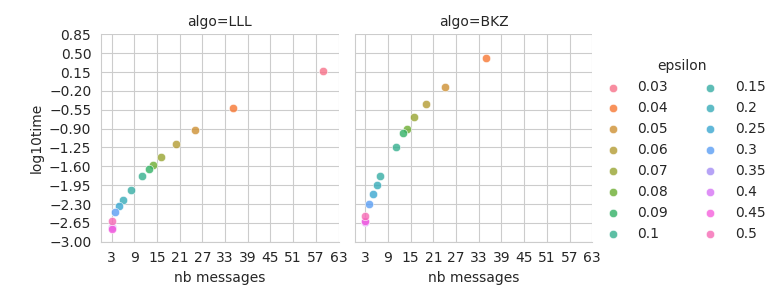
\includegraphics[width=1\linewidth]{img/2048_320_meant_maxm_scatterplots_log.png}
    \caption{Temps moyen et de signatures requises au maximum en fonction de epsilon}
    \label{fig:2048_320_meant_maxm_scatterplots_log}
\end{figure}



\subsection{Expériences avec ECDSA sur P-256}

Nous avons mené l'attaque sur la courbe $P-256$ standardisée par le NIST. Nous avons aussi utilisé LLL et ses variantes comme fpLLL ainsi que BKZ et ses variantes exploité précédemment. Dans le cadre de BKZ, nous avons voulu observer comment évolue cet algorithme lorsque l'on modifie la taille des blocs $\beta$ sans affiner le choix.\smallbreak

Voici un tableau qui indique la taille des blocs et le nom associé dans nos graphes :

\begin{table}[H]
    \centering
    \caption{Tableau de références entre la légende des graphes et $\beta$}
    \begin{tabular}{|c|c|}
        \toprule
        Label & $\beta$\\
        \midrule
        BKZ2-2    & 2 \\
        BKZ2-half & moitié de la matrice\\
        BKZ2-max  & taille de la matrice \\
        \bottomrule
    \end{tabular}
    \label{tab:taille_blocs}
\end{table}

\medbreak

Dans les deux figures ci-dessous (\ref{fig:P-256_meant_meanm_epsi_time} et \ref{fig:P-256_meant_meanm_scatterplots}), on compare les ressources nécessaires en moyenne (temps et signatures) pour faire fonctionner l'attaque. Les paramètres qui influent sur les résultats sont la valeur de epsilon (en nuances de couleurs) et l'implémentation de la réduction de réseau utilisée (indiquée au dessus des graphes).\smallbreak

Nous avons fait le choix représenter des valeurs de epsilon assez faibles que nous avons choisies inférieures à $0.14\%$ car elles sont plus pertinentes pour une attaque réelle. Cependant, nos mesures portent sur des valeurs de epsilon supérieures à $0.4\%$

La machine utilisée pour les expériences suivantes est \ref{jolicoeur}, chaque expérience a été répétée 5 fois.

\begin{figure}[H]
    \centering
    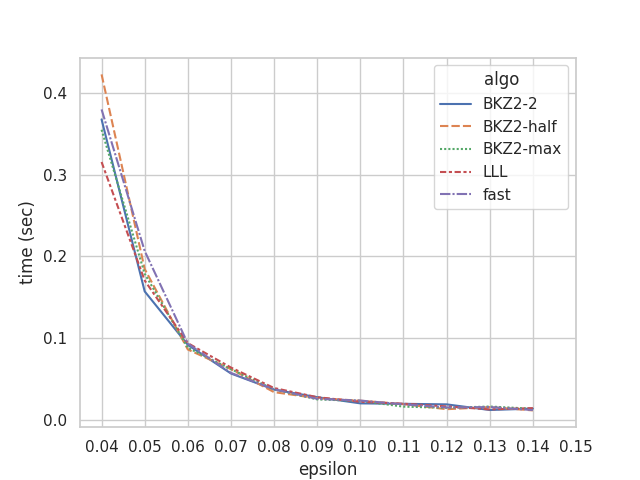
\includegraphics[width=0.75\linewidth]{img/P-256_meant_meanm_epsi_time.png}
    \caption{Temps d'exécution moyen selon l'algorithme et la valeur d'epsilon}
    \label{fig:P-256_meant_meanm_epsi_time}
\end{figure}

Sur cette intervalle de valeurs, les temps d'exécution sont similaires et l'allure des courbes semble similaire.\smallbreak
Cependant, ce résultat est assez différent de ce qui est prévu par la théorie. En effet, LLL et fpLLL sont censés avoir une complexité polynomiale par rapport à la taille du réseau (qui est inversement proportionnelle à la valeur de epsilon).
BKZ est un compromis entre sieving et LLL, par conséquent sa complexité est sous-exponentielle. Par conséquent, si l'on poussait les expériences avec des valeurs de epsilon plus faibles alors on s'attendrait à voir BKZ2-max exploser suivi par BKZ2-half puis BKZ-2. Les résultats suivants ne permettront pas non plus d'observer cette tendance.

\newpage
\begin{figure}[ht]
    \centering
    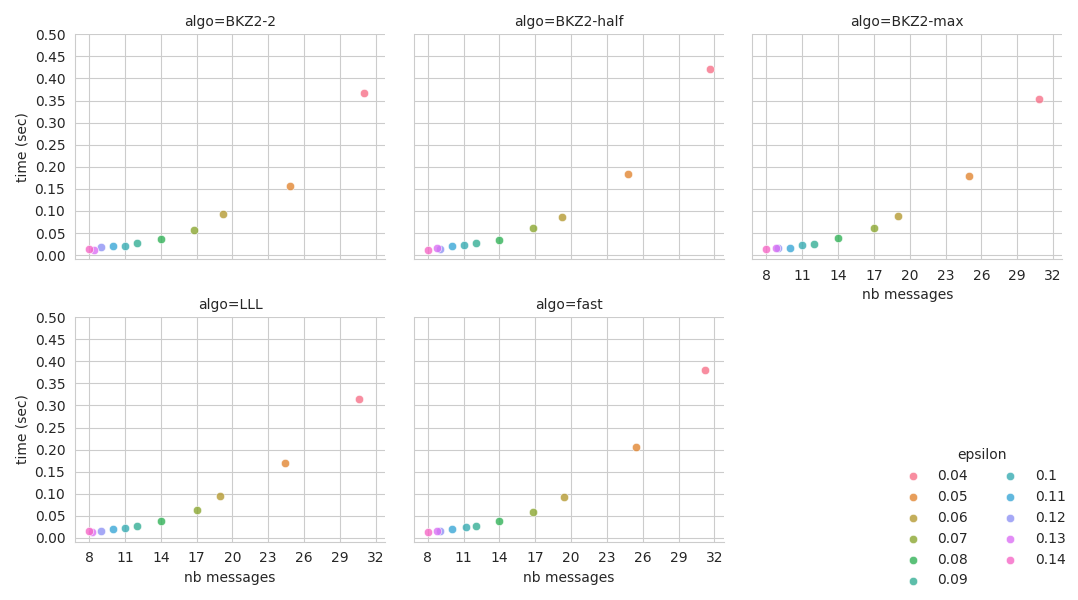
\includegraphics[width=1\linewidth]{img/P-256_meant_meanm_scatterplots.png}
    \caption{P-256 temps moyen et moyenne des signatures requises}
    \label{fig:P-256_meant_meanm_scatterplots}
\end{figure}

Sur cette figure \ref{fig:P-256_meant_meanm_scatterplots}, nous pouvons voir que le nombre de messages requis pour mener l'attaque est similaire selon les algorithmes utilisés. Nous avons trop peu de valeurs pour avancer une statistique précise sur le sujet. Cependant, nous avons observé des expériences réussies avec quelques signatures en moins pour LLL ce qui est du à des heuristiques un peu plus performantes selon nous. Une nouvelle fois, la théorie dit que le facteur d'approximation est meilleur pour BKZ avec de grandes tailles de bloc ce qui amènerait à des attaques réussies avec moins de signatures pour des réseaux de plus grande taille.

\begin{figure}[H]
    \centering
    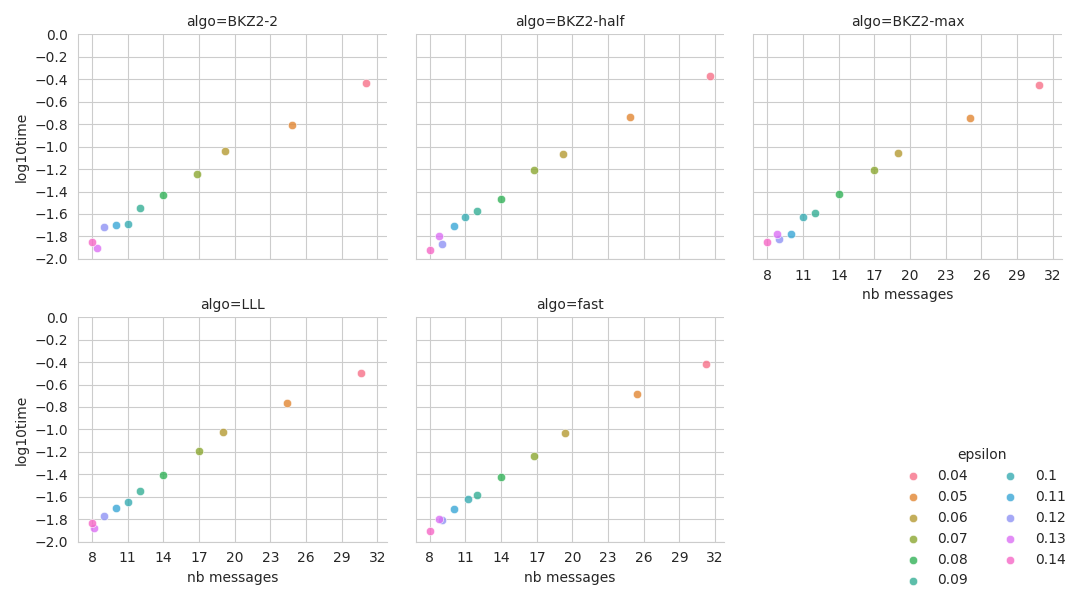
\includegraphics[width=1\linewidth]{img/P-256_meant_meanm_scatterplots_log.png}
    \caption{P-256 moyennes des temps d'exécution en secondes et du nombre de signatures requises (échelle $log_{10}$)}
    \label{fig:P-256_meant_meanm_scatterplots_log}
\end{figure}

Les valeurs les plus grandes de epsilon (entre $0.12$ et $0.14$) semblent se chevaucher sur le graphique \ref{fig:P-256_meant_meanm_scatterplots_log}, comme on utilise une moyenne sur les temps d'exécution et le nombre de signatures requises, on a une certaine sensibilité aux valeurs extrêmes. En effet, si une signature supplémentaire a été nécessaire pour récupérer la clé privée pour une certaine instance du problème alors le point résultant de la moyenne sera légèrement décalé vers la droite.\smallbreak
Nous pourrions augmenter le nombre de mesures pour atténuer cette effet, enlever les valeurs extrêmes ou bien utiliser une médiane.

Voici des tableaux réalisés à partir d'un nouveau jeu de données calculées sur \ref{jolicoeur}. %_2025_02_04_10_52


\begin{center}
    \begin{table}[H]
        \centering
        \caption{Évaluation des performances entre les algortihmes LLL et BKZ de l'attaque de la courbe P-256}
        \label{tab:p-256_LLL_BKZ}
        
        \begin{tabular}{|c|c|cc|cc|}
            \toprule
            Epsilon & Bits connus & \multicolumn{2}{|c|}{LLL} & \multicolumn{2}{|c|}{BKZ} \\
            \cmidrule{3-6}
            & & Temps & Nb signature & Temps & Nb signature  \\
            \midrule
             0.05 &26 & 0.7127 & 26 & 4.954 & 26\\
             0.1  &11 & 0.1256 & 11 & 0.418 & 12\\
             0.15 & 8 & 0.0589 & 8 & 0.1191 & 7 \\
             0.2  & 6 & 0.0459 & 6 & 0.0756 & 6 \\
             0.25 & 5 & 0.0379 & 5 & 0.0492 & 5 \\
             0.3  & 4 & 0.0276 & 4 & 0.0316 & 4 \\
             0.35 & 3 & 0.0173 & 3 & 0.0194 & 3 \\
             0.4  & 3 & 0.0172 & 3 & 0.0191 & 3 \\
             0.45 & 3 & 0.0199 & 3 & 0.0194 & 3 \\
             0.5  & 3 & 0.0138 & 3 & 0.0191 & 3 \\
               
            \bottomrule
        \end{tabular}
    \end{table}
\end{center}



On voit que BKZ performe moins bien que LLL pour les valeurs de epsilon présentées, ce qui est représentatif de ce que nous avons obtenu sur l'ensemble des résultats.
\commentaire{

\subsection{Remarques}

Il semblerait que les limites de l'attaque sont très corrélées avec la taille du réseau que l'on doit réduire. On dépasse le dixième de seconde de calcul quand epsilon est de l'ordre de 0.05 et comme le temps de calcul semble augmenter exponentiellement, nous avons eu des difficultés pour obtenir des résultats pour des valeurs de epsilon inférieures à 0.025.

%Ce résultat est pertinent car la cryptologie sur les réseaux euclidiens ont étés mis sur le devant de la scène lors des compétions organisées par le NIST pour sélectionner les nouvelles normes pour la cryptologie post-quantique.

}


% -------------------------------------------------------------------------------
%
% Conclusion
%
% -------------------------------------------------------------------------------
\newpage
\section{Conclusion}

Notre travail de recherche s'est concentré sur l'article \cite{latAtk}. Une méthode historique d'attaque par canal auxiliaire de DSA qui permet facilement de retrouver la clé secrète utilisée à partir de traces de bonnes qualité et de quelques signatures. Nous l'avons implémenté avec les paramètres de l'époque à l'aide des ressources proposées par le logiciel Sagemath, puis étendu à ECDSA. On a constaté que le passage de 160bits à 256bits rallonge évidemment les temps de calcul mais ne réduit pas les probabilités de réussite pour une même proportion de bits connus. De plus, les différents algorithmes de réduction de réseau que l'on a testé n'ont pas menés à des résultats significativement différents. \medbreak

Nous tenons à rappeler que DSA est considéré comme un standard obsolète au jour de la rédaction de ce rapport. 
%OpenSSH annonce enlever le support DSA pour SSH courant 2025. De manière générale, il est préférable d'utiliser les courbes elliptiques standardisées pour faire de la signature.


\section{Ouverture} \label{sec:ouverture}

Dans cette section, nous allons couvrir différents points de l'attaque où nous pensons qu'il est possible d'apporter des améliorations.


rapidement des améliorations de cette attaque, notamment celle que l'on peut retrouver dans \cite{improvedECDSA}.

\subsection{Avancées sur l'implémentation ECDSA}

Les systèmes cryptographiques ont souvent besoin d'élever certains éléments à une grande puissance, il est donc intéressant de savoir comment réaliser ce calcul le plus rapidement possible. \citetitle{fast_exp_method} \cite{fast_exp_method} présente les meilleures méthodes pour la mise à l'exponentielle.

L'encodage NAF (Non-Adjacent Form) est une représentation particulière des nombres qui permet de réduire le nombre de multiplications, notamment dans les courbes elliptiques. En utilisant des coefficients non adjacents, on minimise le nombre d'opérations coûteuses. Par exemple, la forme 1-NAF garantit qu'il n'y a pas deux coefficients non nuls adjacents, ce qui réduit le nombre de multiplications par rapport à la représentation binaire standard. Les formes 2-NAF et 3-NAF étendent ce concept en permettant des coefficients plus grands, ce qui peut encore réduire le nombre d'opérations nécessaires.

\begin{center}
    \begin{table}[htbp]
        \caption{Tableau de Conversion entre Différentes Formes NAF}
        \label{tab:comparaison_NAF}
        \centering
        \begin{tabular}{|l|cccc|}
            \toprule
            \textbf{Décimal} & \textbf{Binaire} & \textbf{1-NAF} & \textbf{2-NAF} & \textbf{3-NAF} \\
            9 & 1001 & $1001$ & $1 0 0 1$ & $1 0 0 0 (-7)$ \\
            11 & 1011 & $1 0 (-1) 0 (-1)$ & $1 0 0 3$ & $1 0 0 0 (-5)$ \\
            29 & 11101 & $1 0 0 (-1) 0 1$ & $1 0 0 0 0 (-3)$ & $1 0 0 0 0 (-3)$ \\
            42 & 101010 & $101010$ & $3 0 0 (-3) 0$ & $1 0 0 0 5 0$\\
            85 & 1010101 & $1010101$ & $1 0 0 3 0 0 (-3)$ & $5 0 0 0 5$ \\
            170 & 10101010 & $10101010$ & $1 0 0 3 0 0 (-3) 0$ & $5 0 0 0 5 0$ \\
            \hline
        \end{tabular}
    \end{table}
\end{center}

En revanche, une implémentation sous cette forme permet une nouvelle gamme d'attaques par canal auxiliaire, de la même manière que l'attaque \textit{Bellcore} \cite{Bellcore}. Celles-ci ont été étudiées notamment ici \citetitle{wNaf_attack} \cite{wNaf_attack}.

\subsection{Avancées sur la réduction de réseau}

Un autre point clé de l'attaque que l'on a étudié repose sur des algorithmes de réduction de réseau. Nous avons pu tester LLL et BKZ, implémentés sur \textit{Sagemath}. Nous avons aussi pu découvrir \textbf{Flatter} \cite{flatter}, développé dans \citetitle{flatter}, il a été implémenté dans le logiciel de calcul mathématique \textit{pari-GP}. Voici un tableau de comparatifs de leurs résultats \ref{tab:flatter}.

\begin{center}
    \begin{table}[H]
        \caption{Tableau de comparaison des tailles de réseau après application de Flatter, LLL et une étude antérieure}
        \label{tab:flatter}
        \centering
        \begin{tabular}{|c|c|c|c|c|}
        \hline
        \textbf{Dimension} & \textbf{Nombre de bits} & \textbf{fpLLL (s)} & \textbf{\cite{ref32}} & \textbf{\cite{flatter}} \\
        \hline
        128 & 100000 & 3831 & 400 & 69 \\
        \hline
        256 & 10000 & 2764 & 200 & 83 \\
        \hline
        384 & 10000 & 10855 & 780 & 246 \\
        \hline
        \end{tabular}
    \end{table}
\end{center}

Cet algorithme de réduction est très performant, en revanche, comme on peut le voir avec la taille des dimensions, il semble hors-propos de notre cadre. Nous avons pu voir en section \ref{sec:epreuves} que nos réseaux n'atteignaient pas des dimensions de plus de XXX.


Nous avons aussi pu découvrir une amélioration de LLL, nommée L4, \citetitle{l4} \cite{l4}. Celle-ci, encore en développement, semble se combiner à BKZ pour améliorer les réductions de matrices. Nous vous présentons ici un de leurs résultats montrant l'avantage de cette méthode pour l'amélioration des attaques sur ECSA.

\begin{figure}[H]
    \centering
    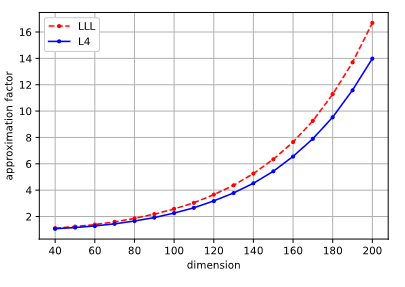
\includegraphics[scale = 0.5]{img/LLL&L4.png}
    \caption{Moyenne du facteur d'approximation $\gamma$}
    \label{fig:LLL&l4}
\end{figure}

Des expériences restent encore à réaliser pour observer l'efficacité réelle de L4. Leur conclusion présente le gain effectif sur LLL, en revanche, l'hybridation de cette solution avec BKZ n'est pas satisfaisante et reste à améliorer.


\subsection{Performance dans la conception du réseau}

Dans \cite{improvedECDSA}, les auteurs utilisent des algorithmes de réduction de réseau et des techniques de criblage avec prédicat. Ils améliorent les travaux précédents en proposant un algorithme de prédicat plus efficace et en combinant le criblage avec des techniques avancées comme "dimensions for free" et "progressive sieving". \smallbreak

Les résultats expérimentaux montrent que leur algorithme surpasse les records existants en termes de temps d'exécution, de nombre d'échantillons et de probabilité de succès. Ils réussissent également à casser des records de réseau précédemment considérés comme infaisables, notamment pour des courbes de 384 bits avec une fuite de 3 bits de clé éphémère et des courbes de 256 bits avec une fuite de 2 bits de clé éphémère. Enfin, ils présentent la première attaque par réseau contre ECDSA avec une fuite de clé éphémère d'un seul bit, permettant de casser une courbe de 112 bits en temps pratique.

Ces avancées démontrent des progrès significatifs dans le domaine des attaques par canal auxiliaire sur la signature ECDSA, ouvrant de nouvelles perspectives pour la recherche en cryptanalyse.

\begin{center}
    \begin{table}[H]
    \centering
    \caption{Comparaison avec les précédents records des attaques par réseau sur (EC)DSA. Chaque colonne correspond à la taille des courbes et chaque ligne correspond au nombre de bits de fuite de clé éphémère par signature.}
    \label{table:comparaison}
    \begin{tabular}{|c|c|c|c|c|}
    \hline
     & \textbf{4-bit} & \textbf{3-bit} & \textbf{2-bit} & \textbf{1-bit} \\
    \hline
    \textbf{112-bit} & - & - & - & \cite{improvedECDSA} \\
    \hline
    \textbf{160-bit} & - & [2002] & [2013], [2021], [2022] & $/$ \\
    \hline
    \textbf{256-bit} & [2019], [2020] & [2021], [2022] & \cite{improvedECDSA} & $/$ \\
    \hline
    \textbf{384-bit} & [2021], [2022] & \cite{improvedECDSA} & $/$ & $/$ \\
    \hline
    \end{tabular}
    
    \end{table}
\end{center}


%-------- Annexes --------
\newpage
\section{Annexes}

\subsection{Babai et Kannan} \label{annexe:Babai}

CVP est en général utilisé dans sa version 'approximation'. Plutôt que de chercher le vecteur de $L$ qui minimise la distance, on cherche un vecteur dont la distance à notre cible est inférieure à un certain $\gamma$. L'algorithme du plan proche de Babai utilise l'algorithme LLL pour résoudre le \(\gamma\)-CVP avec \(\gamma = 2\left(\frac{2}{\sqrt{3}}\right)^d\), où \(d\) est le rang du réseau.

Étant donné une base \(\mathcal{B} \in \mathbb{Z}^{d \times n}\) et un vecteur cible \(t \in \mathbb{Z}^n\), l'algorithme de Babai effectue une réduction de réseau avant de projeter itérativement \(t\) sur chaque vecteur de base réduit successif. La projection arrondie est ensuite soustraite de \(t\) pour obtenir un nouveau vecteur plus proche du point du réseau. L'algorithme de Kannan 

Voici les trois algorithmes mis à notre disposition par la librairie \textit{Sagemath}, nous avons utilisé les trois pour effectuer nos recherches de clés secrètes et effectué des comparaisons de leur efficacité. \medbreak

\textbf{Entrée :} Une base de réseau \(\mathcal{B} \in \mathbb{Z}^{d \times n}\) et un vecteur cible \(t \in \mathbb{Z}^n\).

\textbf{Sortie :} Un vecteur \(x \in L(\mathcal{B})\) tel que \(\forall y \in L(\mathcal{B})\), \(\|x - t\| \leq \gamma \|y - t\|\).
\medbreak


\begin{algorithm}
\caption{Algorithme du Plan Proche de Babai}
\begin{algorithmic}[1]
\Require \(\mathcal{B} \in \mathbb{Z}^{d \times n}\), \(t \in \mathbb{Z}^n\)
\Ensure \(x \in L(\mathcal{B})\) tel que \(\|x - t\| \leq \gamma \cdot dist(t, L(\mathcal{B}))\)
\State Exécuter \(\delta\)-LLL sur \(\mathcal{B}\) avec \(\delta = \frac{3}{4}\)
\State \(b \gets t\)
\For{\(j = n\) to \(1\)}
    \State \( b \gets b - c_j \tilde{b}_j \) où \( c_j \leftarrow \left\lfloor \frac{\langle b, \tilde{b}_j \rangle}{\langle \tilde{b}_j, \tilde{b}_j \rangle} \right\rceil \)
\EndFor
\State \textbf{Retourner} \(t - b\)
\end{algorithmic}
\end{algorithm}


\begin{algorithm}
\caption{Algorithme d'Arrondi de Babai}
\begin{algorithmic}[1]
\Require \(\mathcal{B} \in \mathbb{Z}^{d \times n}\), \(t \in \mathbb{Z}^n\)
\Ensure \(x \in L(\mathcal{B})\) tel que \(\|x - t\| \leq \gamma \cdot dist(t, L(\mathcal{B}))\)
\State Résoudre le système \(x \cdot \mathcal{B} \cdot \mathcal{B}^T = t \cdot \mathcal{B}^T\)
\State \(x \gets \text{arrondi}(x)\)
\State \textbf{Retourner} \(x \cdot \mathcal{B}\)
\end{algorithmic}
\end{algorithm}

\begin{algorithm}
\caption{Algorithme de Kannan}
\begin{algorithmic}[1]
\Require \(\mathcal{B} \in \mathbb{Z}^{d \times n}\), \(t \in \mathbb{Z}^n\)
\Ensure \(x \in L(\mathcal{B})\) tel que \(\|x - t\| \leq \gamma \cdot dist(t, L(\mathcal{B}))\)
\State Construire la matrice \(L\) en ajoutant une ligne et une colonne à \(\mathcal{B}\)
\State \(L \gets \begin{pmatrix} \mathcal{B} & t \\ 0 & \text{weight} \end{pmatrix}\) où \(\text{weight} = \|\mathcal{B}_{-1}\| + 1\)
\State Exécuter LLL sur \(L\)
\For{chaque vecteur \(v\) dans les lignes de \(L\)}
    \If{\(|v[-1]| = \text{weight}\)}
        \State \textbf{Retourner} \(t - v[:-1] \cdot \text{sign}(v[-1])\)
    \EndIf
\EndFor
\State \textbf{Erreur} : Aucun vecteur approprié trouvé dans la base.
\end{algorithmic}
\end{algorithm}

\newpage
\subsection{Développement équations}\label{annexe:Developpement}

$ m_{i} \equiv b y_{i}-x f\left(g^{y_{i}}\right) \quad(\bmod p)$  \\
$ \Leftrightarrow -b y_{i}+x f\left(g^{y_{i}}\right) + m_{i} = 0 \quad(\bmod p)$\\
$ \Leftrightarrow y_{i}+x f\left(g^{y_{i}}\right) (-b)^{-1} + m_{i}(-b)^{-1} = 0 \quad(\bmod p)$\\

Ainsi, on peut simplifier, dans un premier temps,  ces équations en définissant $ A_{i} =  f\left(g^{y_{i}}\right) (-b)^{-1}$ et $ B_{i} = m_{i}(-b)^{-1}$. On obtient nos équations sous la forme :

$$ y_{i}+x A_{i} + B_{i} = 0 \quad(\bmod p)$$

Ensuite, on souhaite faire disparaître la variable \textit{x} de notre ensemble d'équations. Elle correspond à la clé secrète d'Alice et on a admis notre absence d'information sur celle-ci: \\
$ y_{h}+x A_{h} + B_{h} = 0 \quad(\bmod p)$\\
$ \Leftrightarrow x A_{h}= -y_{h} - B_{h} \quad(\bmod p)$\\
$ \Leftrightarrow x = -y_{h}A_{h}^{-1} - B_{h}A_{h}^{-1} \quad(\bmod p)$\\

Maintenant que \textit{x} est simplifié, on va pouvoir faire le pivot de Gauss décrit dans la section \ref{Stratégie de l'attaque}.
Donc : \\$ y_{i}+(-y_{h}A_{h}^{-1} - B_{h}A_{h}^{-1})A_{i} + B_{i} = 0 \quad(\bmod p)$\\
$ \Leftrightarrow y_{i}+-y_{h}A_{h}^{-1}A_{i} - B_{h}A_{h}^{-1}A_{i} + B_{i} = 0 \quad(\bmod p)$\\
On va à nouveau simplifier notre équation en définissant $ A^{\prime}_{i} = A_{h}^{-1}A_{i}$ et $ B^{\prime}_{i} = - B_{h}A_{h}^{-1}A_{i} + B_{i} $, ce qui nous rend avec \ref{eq:milieu} : $y_{i} + y_{h} * A^{\prime}_{i} + B^{\prime}_{i} = 0 \quad(\bmod p)$\\

Enfin, on va intégrer l'information que l'on a pu récupérer de notre attaque par canal auxiliaire. Donc, chaque équation est modifiée pour présenter le changement :\\
$ \alpha_{i}^{\prime}+2^{\lambda_{i}} z_{i}+2^{\mu_{i}} \alpha_{i}^{\prime \prime} + (\alpha_{h}^{\prime}+2^{\lambda_{h}} z_{h}+2^{\mu_{h}} \alpha_{h}^{\prime \prime}) * A^{\prime}_{i} + B^{\prime}_{i} = 0 \quad(\bmod p)$\\
$ \Leftrightarrow 2^{\lambda_{i}} z_{i} + (\alpha_{h}^{\prime}+2^{\lambda_{h}} z_{h}+2^{\mu_{h}} \alpha_{h}^{\prime \prime}) * A^{\prime}_{i} + B^{\prime}_{i}+\alpha_{i}^{\prime}+2^{\mu_{i}} \alpha_{i}^{\prime \prime} = 0 \quad(\bmod p)$ \\
$ \Leftrightarrow z_{i}2^{\lambda_{i}}  +z_{h}2^{\lambda_{h}} A^{\prime}_{i} + (\alpha_{h}^{\prime}+2^{\mu_{h}} \alpha_{h}^{\prime \prime})A^{\prime}_{i} + B^{\prime}_{i}+\alpha_{i}^{\prime}+2^{\mu_{i}} \alpha_{i}^{\prime \prime} = 0 \quad(\bmod p)$\\
$ \Leftrightarrow z_{i}2^{\lambda_{i}}  +z_{h}2^{\lambda_{h}} A^{\prime}_{i} +(\alpha_{h}^{\prime}+2^{\mu_{h}} \alpha_{h}^{\prime \prime})A^{\prime}_{i} + B^{\prime}_{i}+\alpha_{i}^{\prime}+2^{\mu_{i}} \alpha_{i}^{\prime \prime} = 0 \quad(\bmod p)$\\
$ \Leftrightarrow z_{i}  +z_{h}2^{\lambda_{h}} A^{\prime}_{i}2^{-\lambda_{i}} +((\alpha_{h}^{\prime}+2^{\mu_{h}} \alpha_{h}^{\prime \prime})A^{\prime}_{i} + B^{\prime}_{i}+\alpha_{i}^{\prime}+2^{\mu_{i}} \alpha_{i}^{\prime \prime}) 2^{-\lambda_{i}}= 0 \quad(\bmod p)$\\

Ainsi, en définissant $s_{i} = 2^{\lambda_{h}} A^{\prime}_{i}2^{-\lambda_{i}}$ et $ t_{i} =  ((\alpha_{h}^{\prime}+2^{\mu_{h}} \alpha_{h}^{\prime \prime})A^{\prime}_{i} + B^{\prime}_{i}+\alpha_{i}^{\prime}+2^{\mu_{i}} \alpha_{i}^{\prime \prime}) 2^{-\lambda_{i}}$, on obtient enfin nos équations sous forme simplifiée  :
$$  z_{i}+s_{i} z_{h}+t_{i} = 0 \quad(\bmod p)$$

\newpage

\subsection{Considérations matérielles} \label{annexe:machines}

Voici des informations succinctes sur les ordinateurs utilisés pour réaliser les expériences.
Toutes les expériences ont été menées sur place ou en ssh avec le système d'exploitation Debian GNU/Linux 12 (bookworm) 64 bits.

% Elles ont été récupérées avec les commandes suivantes ou bien via le site du cremi : \\\url{https://services.emi.u-bordeaux.fr/exam-test/?page=wol}.

\begin{center}
    \begin{table}[ht]
        \centering
        \caption{configurations des machines utilisées}
        \label{tab:configurations}
        \begin{tabular}{|c|c|c|}
            \toprule
            Machine & modèle CPU & RAM (GO) \\
            \midrule
                \makeatletter\def\@currentlabel{jolicoeur}\makeatother
                jolicoeur\label{jolicoeur} & AMD Opteron 6276 & 124 \\
                \makeatletter\def\@currentlabel{bergman}\makeatother
                bergman\label{bergman}  & Intel i9-13900 & 64 \\
                \makeatletter\def\@currentlabel{plomet}\makeatother
                plomet\label{plomet}  & Intel Xeon W-1290 & 64 \\
                \makeatletter\def\@currentlabel{perbosc}\makeatother
                perbosc\label{perbosc}  & Intel Xeon W-1290 & 64 \\
                \makeatletter\def\@currentlabel{lautrec}\makeatother
                lautrec\label{lautrec}  & Intel Xeon E-2236 & 32 \\
                \makeatletter\def\@currentlabel{goya}\makeatother
                goya\label{goya}  & Intel Xeon E-2236 & 32 \\
                %\makeatletter\def\@currentlabel{millet}\makeatother
                %millet\label{millet} & 2x Intel Xeon Gold 5118  & 64 \\
                %\makeatletter\def\@currentlabel{perbosc}\makeatother
                %perbosc\label{perbosc} & Intel Xeon W-1290 & 64 \\
                %\makeatletter\def\@currentlabel{hendrix}\makeatother
                %hendrix\label{hendrix} & Intel Xeon W-1250P & 48 \\
                %\makeatletter\def\@currentlabel{holdsworth}\makeatother
                %holdsworth\label{holdsworth} & Intel Xeon W-1250P & 48 \\
                %\makeatletter\def\@currentlabel{jordan}\makeatother
                %jordan \label{jordan} & Intel Xeon W-1250P & 48 \\
                
                \makeatletter\def\@currentlabel{biot}\makeatother
                biot\label{biot} & Intel(R) Core(TM) i9-12900 & 64 \\
            \bottomrule
        \end{tabular}
    \end{table}
\end{center}

Dans les parties suivantes, on abrège Double Data Rate Random Access Memory en DDR RAM.

\begin{table}[H]
    \centering
    \caption{Comparaison du débit des différents standards DDR RAM\cite{ram}}
    \begin{tabular}{|l|c|c|c|c|}
        \toprule
        & DDR (1998) & DDR2 (2003) & DDR4 (2014) & DDR5 (2020) \\
        \midrule
        Transfer Speed (GB/s) & 2.1–3.2 & 4.2–6.4 & 17–25.6 & 38.4–51.2 \\
        \bottomrule
    \end{tabular}
    
    \label{tab:ddr_comparaison}
\end{table}


Configuration plausible pour l'ordinateur des chercheurs en 1999 :
\begin{itemize}
    \item DDR RAM 256 Megaoctets
    \item Intel Pentium II - 32 bits, cadencé entre 233 et 450 MHz % https://en.wikipedia.org/wiki/Pentium_II
    \item Windows 98 ou distribution utilisant Linux Kernel 2.1.0
\end{itemize}

Le rapport de débit entre la RAM installée dans les machines du CREMI et celle dans l'ordinateur des chercheurs autour de l'an 2000 se situe entre $10$ et $20$.

De plus, la capacité et la performance des mémoires cache ont aussi évoluées entre temps.

La différence entre leurs temps d'exécution et les nôtres (\ref{tab:comparaison_signatures}) repose donc grandement sur l'évolution technologique depuis 2001, cf. les configurations des machines \ref{annexe:machines} utilisées pour l'attaque. \medbreak


%-------- Bibliography --------
\newpage

\section{Bibliographie}


\printbibliography[heading=none]

\end{document}
